\chapter{CNN Features Robustness}

\label{chapter:CNNFeaturesRobustness}

% ----------------

\section{Introduction}
In a previous chapter \ref{chapter:ConvolutionalNeuralNetworks}, we advocate the use of convolutional neural networks to extract features from images. In this chapter, we evaluate the robustness of CNN features against modifications. In a first time, instead of trying to learn an image representation from scratch, we assess the robustness of existing networks trained on an unrelated classification task. The aim being to find an already good representation, according to a specific distance, whose dimensionality would be reduced later. This step is important because we make the hypothesis that an already robust image representation will still stay more robust after a dimensionality reduction than a less robust image representation. Despite breaking our main problem into two sub problems (features extraction and dimensionality reduction) is certainly not optimal, depending on the dimensionality reduction method, it is possible to fine tune the image representation. It is for example possible with methods based on neural networks such as: Minimal Loss Hashing and Triplet Ranking Loss. By optimizing at the same time the image representation and the dimensionality reduction, the retrieval performance should probably be better.

\section{Protocol}
The protocol is inspired from our previous benchmark for Reverse Image Search described in chapter \ref{chapter:Benchmarking}. It is based on a set of images that are modified according to some transformations. We then consider a base image and its modified versions as similar amongst themselves, and all other pairs of images as dissimilar. All images are queried and the average precision, recall and Fmeasure are computed over all queries.

\subsection{Preparation}
Following are the steps to prepare images for the benchmark.

\begin{enumerate}
	\item Select $N$ images that are representative to an application with no duplicated images. In our case, $N$ is equal to either 200, 2500 or 25,000.
	\item Select $K$ modifications and from the $N$ base images, generate $K$ new image sets containing $K \times N$ modified images. In our case $K=6$, and the modifications are those enumerated in section \ref{chapter:Benchmarking:section:Protocol}: blur, grayscale, resize, JPEG compression, rotation and cropping.
	\item With a convolutional neural network, extract the features from all images. More details about this step are given in section \ref{chapter:CNNFeaturesRobustness:section:Models}.
\end{enumerate}

\subsection{Distribution of distances}
To get a rough idea of the robustness of CNN features against modifications, we analyze the distribution of distances between similar and dissimilar images. It is also useful to know the distribution of distances for the RIS benchmark. In fact, we can infer an approximate value for the best radius separating similar and dissimilar images.

\begin{enumerate}
	\item For each modification, compute the distance between each base image and its modified version. Take this distance in account in the computation of the minimum, first quartile, median, last quartile and maximum distance between the base and the modified image set. Draw a box plot with these data.
	\item For each pair of different images in the base image set, compute the distance between them.  Take this distance in account in the computation of the minimum, first quartile, median, last quartile and maximum distance between dissimilar images. Draw a box plot with these data.
\end{enumerate}

The resulting box plots can be seen in the Result section \ref{chapter:CNNFeaturesRobustness:section:Results} of this chapter. Ideally, the distribution of distances should not overlap. In other words, the distances between similar images must be strictly smaller than the distances between dissimilar images.

\subsection{RIS benchmark}
To get a precise idea of the retrieval performance using CNN features, we implement the same benchmark as in chapter \ref{chapter:Benchmarking}. We compute all distances between all pairs of images and apply a threshold below which images are considered as similar. Then we compute the mean precision, the mean recall and the mean F-measure. The protocol is repeated for various threshold, the threshold that maximizes the F-measure can be considered as the best radius for the reverse image search system.

\begin{enumerate}
	\item Make search queries with the $(K+1) \times N$ images from the base and modified sets.
	\item Analyse the search results and compute the mean precision, the mean recall and the mean F-measure of all queries.
	\begin{enumerate}
		\item The relevant results are the $K+1$ images that are the modified version of the query image. Thus, the result of each query should contain K+1 images that come from the same base image as the query image.
	\end{enumerate}
\end{enumerate}

The resulting plots can be seen in the Result section \ref{chapter:CNNFeaturesRobustness:section:Results} of this chapter. More detailed results for \textit{VGG16\_block5\_pool\_max} with Cosine distance are available in appendix \ref{chapter:ResultsVGG16Block5PoolMax}. Ideally, the maximum F-measure should be near to 1.

\section{Models}
\label{chapter:CNNFeaturesRobustness:section:Models}
In this section, we describe all models compared in the benchmark. To extract the features, we use a pretrained neural network to predict the label of an image. The feature vector consists of the activations of the units of one specific layer. If the layer is a convolutional or pooling layer, the results are 2D features maps. In this case, the activations are flattened using a global average or maximum pooling. We compare the models described in section \ref{chapter:ConvolutionalNeuralNetworks:section:Models}: \textit{VGG16}, \textit{VGG19}, \textit{ResNet50}, \textit{InceptionV3}. We also evaluate \textit{Xception}, which is also a model available in Keras. If needed the feature vectors can be normalized to unit length in Euclidean distance. To compare the feature vectors, two distances are used: Euclidean and Cosine. 

In the following sections, we describe, for all models, all layers that we compared. The name of layers are the same as in the Keras library. For the models, the naming convention we use in the program is: [network]\_[layer]. If the feature vector is normalized with L2 we add \textit{\_norm\_l2} at the end. For example, \textit{ResNet50\_flatten\_1\_norm\_l2} is extracted from the \textit{flatten\_1} layer of the \textit{ResNet50} network and is normalized as unit length in Euclidean distance.

\subsection{VGG}
In VGG16 and VGG19, available layers ordered by increasing depth are:
\begin{itemize}
	\item block\{\textit{i}\}\_pool\_avg for $i \in \{3, 4, 5\}$
	\item block\{\textit{i}\}\_pool\_max for $i \in \{3, 4, 5\}$
	\item flatten
	\item fc1
	\item fc2
	\item predictions
\end{itemize}

\subsection{ResNet50}
In ResNet50, available layers ordered by increasing depth are:
\begin{itemize}
	\item activation\_\{\textit{i}\}\_avg for $i \in \{4, 7, 10, 13, 16, 19, 22, 28, 31, 34, 37, 40, 43, 46\}$
	\item activation\_\{\textit{i}\}\_max for $i \in \{4, 7, 10, 13, 16, 19, 22, 28, 31, 34, 37, 40, 43, 46\}$
	\item avg\_pool\_avg
	\item avg\_pool\_max
	\item flatten\_1
	\item predictions
\end{itemize}

\subsection{InceptionV3}
In InceptionV3, available layers ordered by increasing depth are:
\begin{itemize}
	\item mixed\{\textit{i}\}\_avg for $i \in \{0, 1, 2, 3, 4, 5, 6, 7, 8, 9, 10\}$
	\item mixed\{\textit{i}\}\_max for $i \in \{0, 1, 2, 3, 4, 5, 6, 7, 8, 9, 10\}$
	\item predictions
\end{itemize}

\subsection{Xception}
In Xception, available layers ordered by increasing depth are:
\begin{itemize}
	\item add\_\{\textit{i}\}\_avg for $i \in \{1, 2, 3, 4, 5, 6, 7, 8, 9, 10, 11, 12\}$
	\item add\_\{\textit{i}\}\_max for $i \in \{1, 2, 3, 4, 5, 6, 7, 8, 9, 10, 11, 12\}$
	\item block14\_sepconv1\_act\_avg
	\item block14\_sepconv1\_act\_max
	\item block14\_sepconv2\_act\_avg
	\item block14\_sepconv2\_act\_max
	\item predictions
\end{itemize}

\section{Implementation}
Our implementation is on GitHub \footnote{https://github.com/mgaillard/CNNFeaturesRobustness}. It consists of three main programs and a bash script to orchestrate their executions.

The first program is a Python script that extracts features from images using the neural network library Keras \cite{chollet2015keras}. The feature vectors can be saved in HDF5 files, which are then read during the execution of the second and third programs.

The second program is the implementation of the distance benchmark. It computes statistics on the distribution of distances between similar and dissimilar images. Those are first written in a file and then used to generate a plot with gnuplot.

The third program is the RIS benchmark. It is written in C++ with OpenMP, to fasten the computation of distances in high dimensional spaces thanks to multi-threading and SIMD. This benchmark computes the mean precision, recall and F-measure of a RIS system based on the previously extracted features. The results are first written in a file and then used to generate a plot with gnuplot.

The workflow of the bash script is:
\begin{enumerate}
	\item Images are modified according to the $K$ modifications with ImageMagick \footnote{www.imagemagick.org}.
	\item Features are extracted from the $(K+1) \times N$ images according to all possible models.
	\item The distance benchmark is executed for all features according to Euclidean and Cosine distance.
	\item The RIS benchmark is executed for all features according to Euclidean and Cosine distance.
\end{enumerate}

\section{Results}
\label{chapter:CNNFeaturesRobustness:section:Results}

Because the benchmark is compute intensive, to find the best model we proceed in three steps. Firstly, we compare all models with all distances but only with 200 images. We retain only the models whose F-measure is above 90\%. Secondly, we repeat this process with 2,500 images. The best models with 2500 images ordered by decreasing F-measure are:

\begin{itemize} 
	\item \textit{VGG16\_flatten} with Cosine distance; $Fmeasure = 0,952$
	\item \textit{VGG19\_flatten} with Cosine distance; $Fmeasure = 0,949$
	\item \textit{ResNet50\_activation\_46\_max} with Cosine distance; $Fmeasure = 0,948$
	\item \textit{ResNet50\_activation\_43\_max} with Cosine distance; $Fmeasure = 0,941$
	\item \textit{VGG16\_block5\_pool\_max} with Cosine distance; $Fmeasure = 0,931$
	\item \textit{VGG19\_block5\_pool\_max} with Cosine distance; $Fmeasure = 0,929$
	\item \textit{InceptionV3\_mixed9\_max} with Cosine distance; $Fmeasure = 0,918$
	\item \textit{InceptionV3\_mixed9\_avg} with Cosine distance; $Fmeasure = 0,911$
\end{itemize}

Finally, we compare these models with all the 25,000 images from the MIRFLICKR collection.

\subsection{Distribution of distances}
In figure \ref{fig:distributions_VGG16_block5_pool_max_cosine}, we present the distribution of distances obtained with \textit{VGG16\_block5\_pool\_max} with Cosine distance. Only one model is presented because this benchmark is not as precise as the RIS benchmark, and is mainly used to get an idea of the value of the best radius. Moreover, all models have similar distribution of distances.

\begin{figure*}
	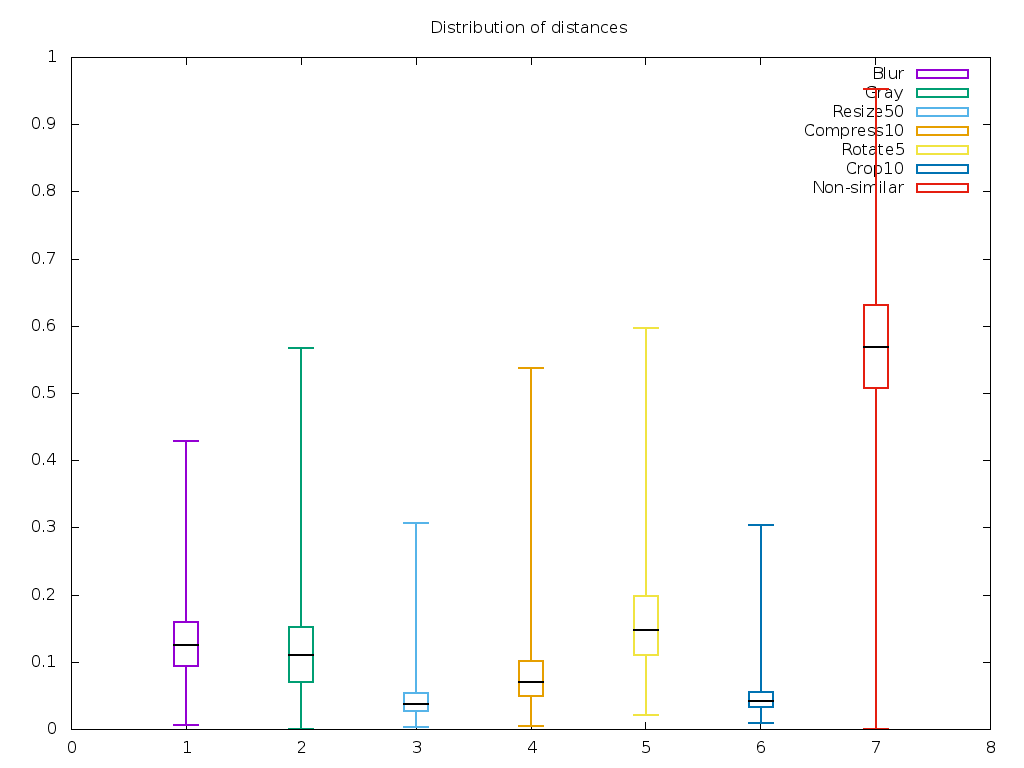
\includegraphics[width=\textwidth]{img/distributions_VGG16_block5_pool_max_cosine.png}
	\caption{Distribution of distances according to a modification obtained with \textit{VGG16\_block5\_pool\_max} with Cosine distance}
	\label{fig:distributions_VGG16_block5_pool_max_cosine}
\end{figure*}

We can see that distances between base and modified images are statistically smaller than the distances between dissimilar images. The interquartile ranges are especially not overlapping, which means that it is possible to differentiate the majority of similar and dissimilar images. The median distance between dissimilar images is about 0.6. If one uses this value as radius for the nearest neighbor search, approximately half of all images would be retrieved. Depending on the modification, the distribution of distances is not the same. Distances between base images and images that are resized to 50\% or cropped by 10\% on the right are smaller than for other modifications. Consequently, we can say that features extracted with \textit{VGG16\_block5\_pool\_max} are more robust to resize and cropping than JPEG compression, grayscale filter, Gaussian blur and rotation.

\subsection{RIS benchmark}

\subsubsection{Retrieval performance against all modifications}
The results of the benchmark with all modifications are shown in table \ref{table:benchmark_all}. Each line represents the maximum F-measure of each model along with the corresponding radius, precision and recall.

\begin{table*}
	\centering
	\caption{Benchmark with all modifications on 25,000 images: maximum Fmeasure}
	\label{table:benchmark_all}
	\begin{tabular}{|crcrrrr|}
	\hline
	Model                         & Dimensions & Distance & Radius & Precision & Recall & Fmeasure \\
	\hline
	VGG16\_flatten                &      25088 & cosine   &   0,51 &     0,954 &  0,943 &    0,936 \\
	VGG19\_flatten                &      25088 & cosine   &   0,50 &     0,955 &  0,934 &    0,931 \\
	ResNet50\_activation\_46\_max &       2048 & cosine   &   0,17 &     0,968 &  0,913 &    0,928 \\
	ResNet50\_activation\_43\_max &       2048 & cosine   &   0,14 &     0,952 &  0,919 &    0,921 \\
	VGG16\_block5\_pool\_max      &        512 & cosine   &   0,23 &     0,947 &  0,898 &    0,904 \\
	VGG19\_block5\_pool\_max      &        512 & cosine   &   0,23 &     0,948 &  0,892 &    0,902 \\
	InceptionV3\_mixed9\_max      &       2048 & cosine   &   0,20 &     0,926 &  0,892 &    0,881 \\
	InceptionV3\_mixed9\_avg      &       2048 & cosine   &   0,20 &     0,924 &  0,865 &    0,866 \\
	\hline
	\end{tabular}
\end{table*}

We can see that despite the fact that the F-measure decreases by about 3 points with 25,000 images compared to 2,500 images, the F-measures are still very good. For comparison, on the same benchmark, the DCT based perceptual hash function yields to a F-measure of about 0.6 (cf. section \ref{chapter:Benchmarking:section:Results}).

\subsubsection{Retrieval performance against single modification}
The results of the benchmark with single modifications are shown in table \ref{table:cnn_benchmark_single} and in figure \ref{fig:cnn_benchmark_single}. Each bar represents the maximum F-measure of each model against a single modification. The radius at which the F-measure is maximum can vary depending on the model and the modification. Thus, this figure gives an idea of the best retrieval accuracy against a single modification. This is why individually the F-measure is better than in the benchmark against all modifications. Because in this latter, the radius is the same for all modifications.

\begin{sidewaysfigure*}
	\centering
	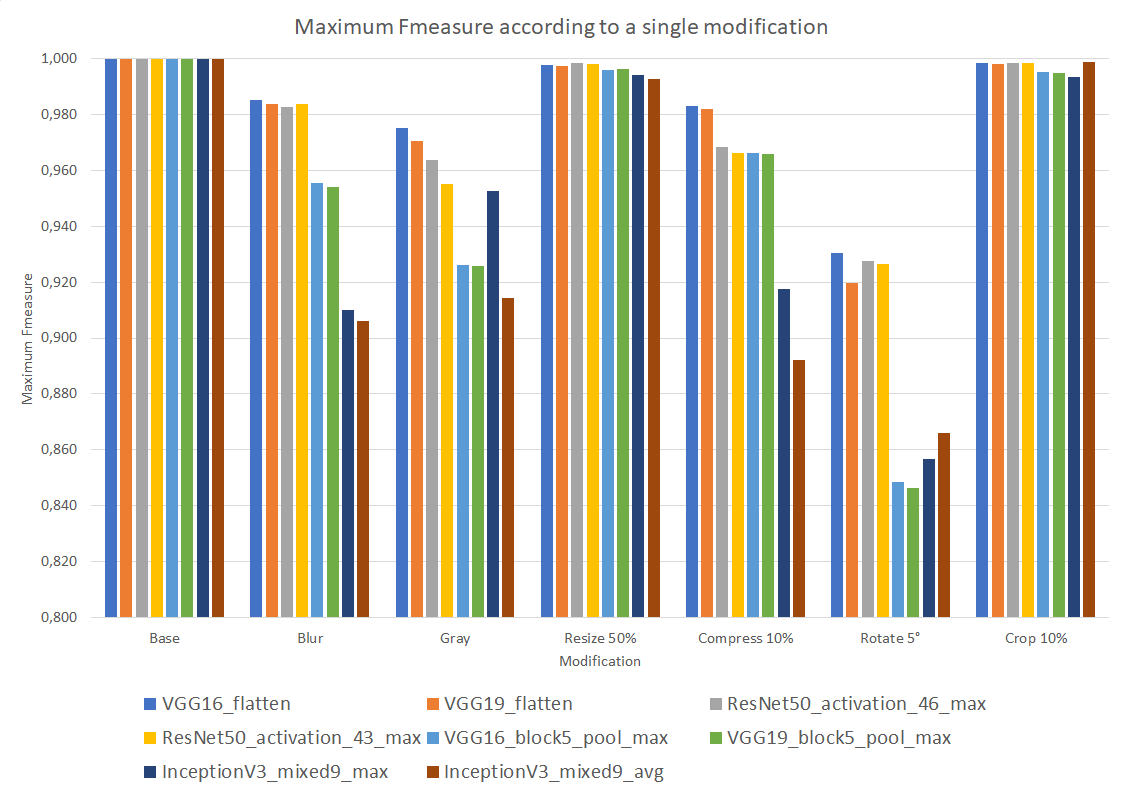
\includegraphics[totalheight=0.7\textheight]{img/cnn_benchmark_single.png}
	\caption{Maximum Fmeasure of CNN models against single modifications}
	\label{fig:cnn_benchmark_single}
\end{sidewaysfigure*}

\begin{table*}
	\begin{tabular}{|l|rrrrrrr|}
    \hline
                                  &  Base &  Blur &  Gray & Resize & Compr & Rotate &  Crop  \\
    \hline                                                                           
    VGG16\_flatten                & 1,000 & 0,985 & 0,975 &  0,998 & 0,983 &  0,930 & 0,998  \\
    VGG19\_flatten                & 1,000 & 0,984 & 0,971 &  0,998 & 0,982 &  0,920 & 0,998  \\
    ResNet50\_activation\_46\_max & 1,000 & 0,983 & 0,964 &  0,998 & 0,968 &  0,928 & 0,998  \\
    ResNet50\_activation\_43\_max & 1,000 & 0,984 & 0,955 &  0,998 & 0,966 &  0,927 & 0,999  \\
    VGG16\_block5\_pool\_max      & 1,000 & 0,955 & 0,926 &  0,996 & 0,966 &  0,848 & 0,995  \\
    VGG19\_block5\_pool\_max      & 1,000 & 0,954 & 0,926 &  0,996 & 0,966 &  0,846 & 0,995  \\
    InceptionV3\_mixed9\_max      & 1,000 & 0,910 & 0,953 &  0,994 & 0,917 &  0,857 & 0,994  \\
    InceptionV3\_mixed9\_avg      & 1,000 & 0,906 & 0,914 &  0,993 & 0,892 &  0,866 & 0,999  \\
    \hline
	\end{tabular}
	\caption{Maximum Fmeasure of CNN models against single modifications. Bar chart in figure \ref{fig:cnn_benchmark_single}.}
	\label{table:cnn_benchmark_single}
\end{table*}

We can see that all models work well and their F-measures are at least above 0.8. All models are very robust against resize to half-size and cropping 10\% on the right, with a F-measure greater than 0.99. The robustness against Gaussian blur, grayscale filter and JPEG compression is good, with a F-measure greater than 0.9. Rotation is the harder modification, with a F-measure of about 0.85 for \textit{VGG16\_block5\_pool\_max}, \textit{VGG19\_block5\_pool\_max}, \textit{InceptionV3\_mixed9\_max} and \textit{InceptionV3\_mixed9\_avg}, and about 0.92 for the others. Models based on \textit{ResNet50} yields to the best results for all modifications.

\subsection{Conclusion}
The objective of this chapter is to find an image representation that is robust against modifications. In chapter \ref{chapter:Benchmarking}, we compare different perceptual hash functions, which can be used as image representation, and show that they are not robust against cropping and rotation. In this chapter, we compare features extracted with off the shelf convolutional neural networks and find a set of models that have very good retrieval performances against modifications. Especially, these are quite robust against rotation and very robust against cropping. 

Robustness is certainly caused by preprocessing and data augmentation during training. Because the input of the convolutional neural network has always a constant size, images are first resized, thus features are robust against scaling. During training, it is common to generate more samples by transforming original images. For example, during the training of VGG \cite{simonyan2014verydeep}, to obtain the fixed size input images, training images are randomly cropped from rescaled training images. Therefore, the neural network is forced to learn a representation that is robust against cropping. More generally, by choosing the modifications made during the data augmentation step, one could give the neural network the ability to be robust against these modifications.

Two different distances are used to compare feature vectors: Euclidean and Cosine. However, it appears that cosine distance yields better results than Euclidean distance. We suppose that it is because, with convolutional neural networks, a neuron is activated with the presence of a feature. The level of presence of the feature is not as important as the fact that it is present.

Of course, CNN features are very robust against modifications but they are not suited for large scale applications. Indeed, the dimensionality of CNN feature vectors is very high. For more details, see the dimensions column of table \ref{table:benchmark_all}. As explained in chapter \ref{chapter:ReverseImageSearch}, it is currently impossible to index $p$-dimensional feature vectors when $p$ is greater than 20. For a large-scale application, one should reduce the dimension of the CNN feature vectors. In the next chapter, we present a method to map feature vectors into binary codes that preserve similarity.